
\section{Jackson vs. Gson}

When a choice had to be made for the JSON parsing library for this project, two
libraries came to mind: Jackson and GSON.\newline

Jackson is a project started in 2008 by Tatu Saloranta and Paul Brown. It has
gained popularity for it's features and fast serialization and deserialization
times.\newline

GSON is a project started in 2008 by Google. It has always been in direct
competition both for features and speed with Jackson.\newline

Some searches have been made for benchmarks for the two libraries. A few
blogs\cite{jacksonvsgson} \cite{jacksonvsgson2} \cite{jacksonvsgson4} and the
wiki entries for a few benchmarking tools\cite{jacksonvsgson3} \cite{jacksonvsgson5}
have been used as guidelines. The author has also tried out and weighted his
subjective opinion on the use of both libraries for simple serializing and
deserializing of JSON messages. The conclusions are as follows:
\begin{enumerate}
  \item \textbf{Features} - Although for the specific needs of this project,
  advanced features were not necessary, this criteria has been considered. A
  six part article on the blog programmerbruce.blogspot.de compares the features
  of GSON and Jackson and deems Jackson the better library.
  
  \item \textbf{Speed} - A test done in 2009 by Tatu Saloranta on his blog
  \url{http://www.cowtowncoder.com/blog/archives/2009/09/entry_326.html}, one of
  the two who started the Jackson project, deemed it much faster than GSON, as
  seen in Figure\ref{fig:jacksonvsgson1}. 'Tps' is \begin{quote}number of
  documents read, written, or read-modify-written per second\end{quote}
   
  \begin{figure}
  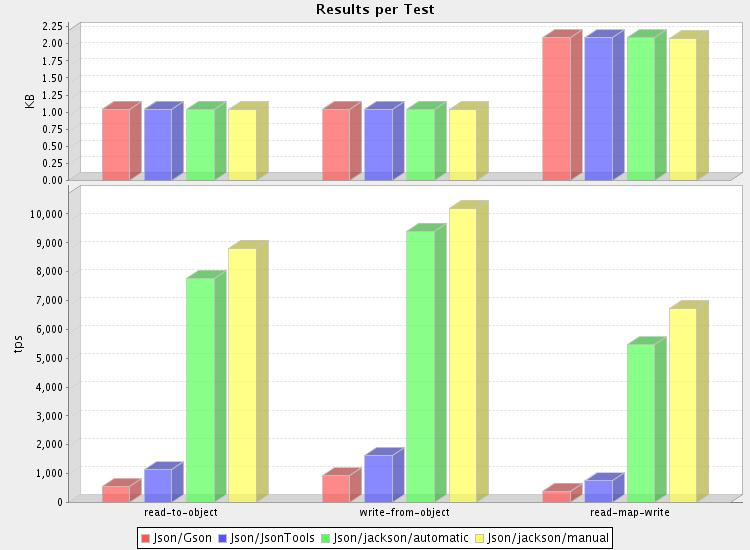
\includegraphics[height=3.5in,width=6.23in]{./images/benchmarks/testcase0.jpg}
  \caption{\small \sl Jackson vs Google-gson vs BerliOS
  (\textbf{\url{http://www.cowtowncoder.com/perf/json-bind-2009-09-23/testcase0.jpg}})}
  \label{fig:jacksonvsgson1}
  \end{figure}
  
  Another test has been done and published in a wiki entry of json-benchmark,
  in 2011. Android's Dalvik's ParseBenchmark.java has been used to benchmark
  the libraries. The results yielded have been:\newline
  \begin{verbatim}
                          TWEETS                              
           api run   ms linear runtime                    % 
ANDROID_STREAM   B 28.8 =================              207% 
JACKSON_STREAM   B 13.9 ========                       100% 
   GSON_STREAM   B 33.1 ===================            238% 
      ORG_JSON   B 36.2 =====================          260% 
     JSON_MINI   B 50.0 ============================== 360% 

                         READER_SHORT                        
           api run    ms linear runtime                    % 
ANDROID_STREAM   B  6.78 ================               177% 
JACKSON_STREAM   B  3.82 =========                      100% 
   GSON_STREAM   B  7.07 ================               185% 
      ORG_JSON   B  7.61 ==================             199% 
     JSON_MINI   B 12.49 ============================== 327% 

                        READER_LONG                         
           api run   ms linear runtime                    % 
ANDROID_STREAM   B 69.6 =====================          254% 
JACKSON_STREAM   B 27.4 ========                       100% 
   GSON_STREAM   B 68.1 =====================          248% 
      ORG_JSON   B 68.9 =====================          251% 
     JSON_MINI   B 95.0 ============================== 347% 
  \end{verbatim}  -
  \textbf{\url{https://code.google.com/p/json-benchmark/wiki/AndroidBenchmarks}}\newline
   
  A third test done in 2012 has been found on \url{blog.novoj.net}, where a
  multitude of libraries including Jackson 2.0.4 and GSON 2.1 were tested. This
  test also deems Jackson as faster at serializing/deserializing, as seen in
  Figure\ref{fig:jacksonvsgson2}.\newline
  
  \begin{figure}
  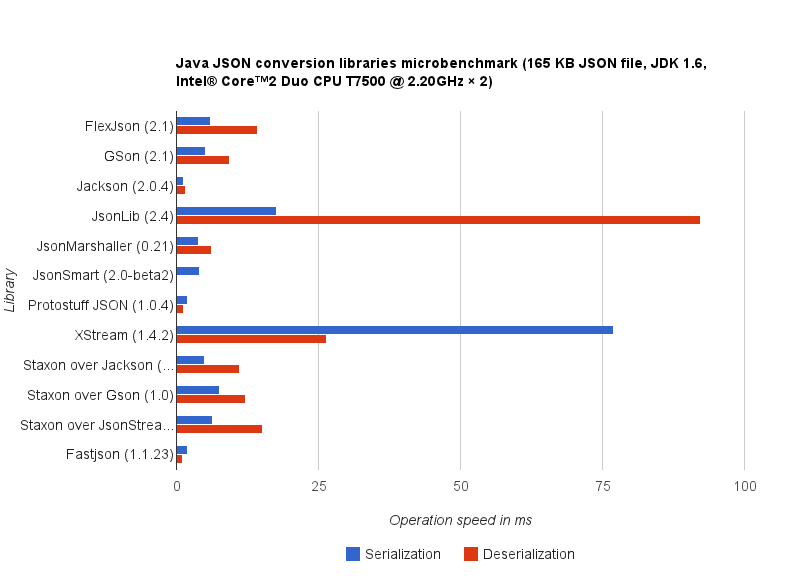
\includegraphics[height=4.5in,width=6.23in]{./images/benchmarks/oimg.png}
  \caption{\small \sl Jackson vs GSON in a comparison over multiple libraries
  (\textbf{\url{http://blog.novoj.net/2012/02/05/json-java-parsers-generators-microbenchmark/}})}
  \label{fig:jacksonvsgson2}
  \end{figure}
  
  A fourth test over several features of multiple JSON libraries, found in a
  wiki entry of jvm-serializers that has been last updated in 2013, also deems
  Jackson the fastest.
  
  \item \textbf{Personal choice} Both Jackson and GSON have been tried out
  before choosing one. Jackson has been preferred for it's ease of use and the fact
  that it offers the ObjectMapper, which gives straightforward functionality to
  'peel' layers from the JSON into Java HashMaps. GSON only allows the use of
  POJOs. For a project where changes have occurred often, like the one
  documented in this paper, Jackson was preferred.
  
  
\end{enumerate}

